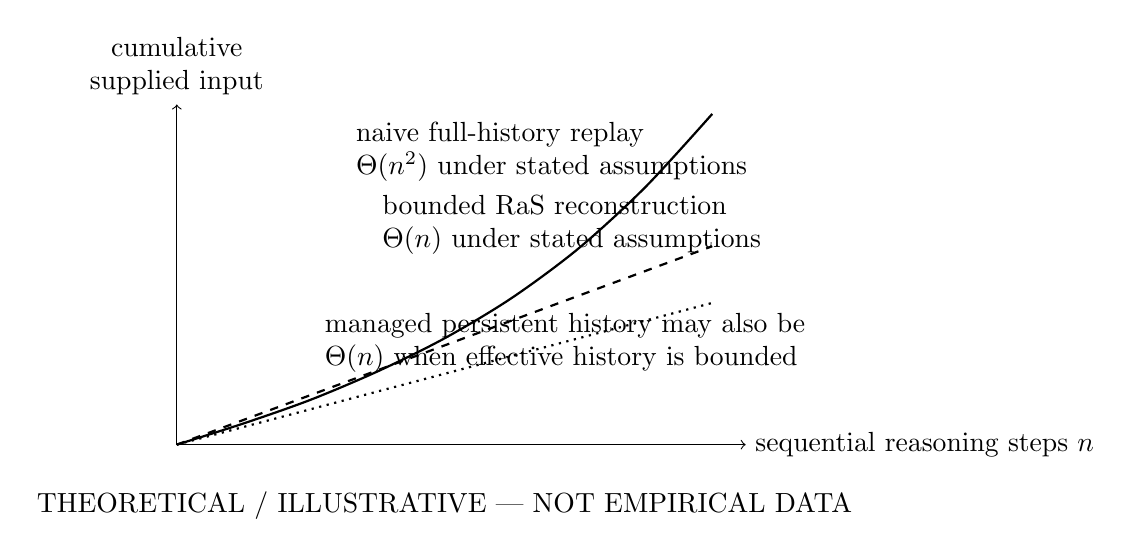
\begin{tikzpicture}[x=0.85cm,y=0.6cm]
\draw[->] (0,0) -- (8.5,0) node[right]{sequential reasoning steps $n$};
\draw[->] (0,0) -- (0,7.2) node[above,align=center]{cumulative\\supplied input};
\draw[thick] plot[smooth] coordinates {(0,0) (1,0.45) (2,0.95) (3,1.55) (4,2.25) (5,3.1) (6,4.15) (7,5.45) (8,7)};
\draw[thick,dashed] (0,0) -- (8,4.2);
\draw[thick,dotted] (0,0) -- (8,3.0);
\node[align=left] at (5.6,6.2) {naive full-history replay\\$\Theta(n^2)$ under stated assumptions};
\node[align=left] at (5.9,4.65) {bounded RaS reconstruction\\$\Theta(n)$ under stated assumptions};
\node[align=left] at (5.8,2.15) {managed persistent history may also be\\$\Theta(n)$ when effective history is bounded};
\node[below,align=center] at (4,-0.8) {THEORETICAL / ILLUSTRATIVE --- NOT EMPIRICAL DATA};
\end{tikzpicture}
